\chapter{IoT}
In questo capitolo andremo a vedere per prima cosa cos'è l'internet delle cose, per poi descrivere la board che abbiamo utilizzato per realizzare il nostro progetto. 

\section{Il futuro delle smart home}
Tutti noi abbiamo sentito parlare, almeno una volta, dell'internet delle cose,
ma in pochi sanno dare una definizione precisa di che cosa sia l'IoT.
Questo perché una definizione rigorosa ad oggi non esiste.
Quello che si intende per Internet of Things è l'estensione della rete ad un numero sempre crescente di dispositivi, o meglio oggetti.
L'insieme di questi: termostati, robot, droni, smart tv, lavastoviglie e molti altri elettrodomestici; rappresenta una solida base per la costruzione di vere e proprie case intelligenti.

L'IoT sta prendendo, giorno dopo giorno, una fetta di mercato sempre più ampia, evolvendosi in fretta e senza seguire standard e protocolli ben specifici. 
Marteen Ector\footnote{Marteen Ectors è uno dei massimi esponenti dell'IoT di  Canonical} ha scritto un articolo\cite{smart} in cui evidenzia dei possibili problemi relativi al futuro di questi oggetti intelligenti.
In particolare si chiede se ci troviamo in una di queste ere:
\begin{itemize}
\item Internet of Useless Things era
\item Internet of Isolated Things era
\item Internet of Insecure Things era
\item Internet of Smart Cheap Things era
\item Internet of App-Enabled Things era
\end{itemize}
Andiamo ad analizzare ogni singola era singolarmente. 
Molti di questi oggetti sono \emph{inutili}, o quasi. Si pensi ad una semplice lampadina, è bello poterla pilotare senza doversi muovere dal divano, ma il problema che risolve è banale.

Non tutti questi smart device parlano la stessa lingua. Prodotti di costruttori diversi usano protocolli diversi \emph{isolandosi} l'un l'altro.

Ci capita spesso di vedere falle di sicurezza che permettano a dei semplici "smanettoni" di accedere senza troppi problemi al microfono e alla webcam della nostra smart tv, anche delle marche più famose.
Siamo sicuri che vogliamo una casa \emph{insicura}?

Il quarto punto rappresenta in realtà un vantaggio dato dal costo delle componenti elettroniche che si sta abbassando drasticamente.
Grazie a ciò è possibile acquistare dei mini-pc per pochi euro. 
Una generica casa, con l'ausilio di questi dispositivi e di qualche sensore, può raccogliere più informazioni di quante ne raccoglieva google 10 anni fa.

Infine, per ogni oggetto che compriamo, troviamo la relativa app sullo store che permette di utilizzare il dispositivo che altrimenti sarebbe inutilizzabile.

Prendendo atto di queste considerazioni e del fatto che il nostro sistema deve adattarsi più all'uso in ufficio che in una casa, abbiamo deciso che il nostro sistema deve avere le seguenti caratteristiche:
\begin{enumerate}
\item \textbf{Open source}: per dare la possibilità a chiunque di migliorarlo e di integrarlo con i propri dispositivi;
\item \textbf{Centralizzato}: non vogliamo avere tanti oggetti intelligenti,
ma uno centrale che ne controlli tanti "stupidi". Questa soluzione non è adatta per spazi ampi come una casa in cui comporterebbe un alto costo per il cablaggio, ma è adatta a singole stanze come un ufficio. 
\end{enumerate} 

\section{Raspberry}
Raspberry è un piccolo calcolatore elettronico dalle dimensioni di una
carta di credito sviluppato nel Regno Unito dalla Raspberry Pi
Foundation. Lo scopo di questa fondazione è quello di sviluppare un
dispositivo economico, che ha la capacità di stimolare l'insegnamento
dell'informatica e della programmazione nelle scuole. La scheda è stata
progettata per ospitare sistemi operativi basati su un kernel linux, tra i
più usati troviamo:
\begin{itemize}
\item Raspbian
\item Ubuntu mate
\item Snappy Ubuntu Core
\item Windows 10 IoT Core
\end{itemize}
Per quanto riguarda i componenti hardware, esso ha la stessa struttura
dei moderni Personal Computer. Raspberry Pi rispetta perfettamente il
modello di Von Neumann, nella quale si individuano quattro componenti
fondamentali: l'unita di elaborazione e controllo, la memoria, il sistema
di ingresso/uscita, il sistema di interconnessione. Inizialmente esistevano tre modelli di Raspberry Pi:
\begin{enumerate}
\item Model A, consigliato per i progetti embedded;
\item Model B, consigliato per l'utilizzo nelle scuole;
\item Model B+, potenziamento del Model B.
\end{enumerate}
Successivamente sono uscite nuove versioni del model B, caratterizzate da più RAM e una CPU migliore, che prendono il nome di Rasperry PI 2 e 3.
Per il nostro progetto abbiamo scelto di utilizzare il Raspberry PI 2 in
quanto è il dispositivo che apre a maggiori possibilità. Il Raspberry Pi 2,
infatti, è dotato di 4 porte USB, un connettore femmina RJ45
10/100BaseT, lettore MicroSD, connettore display DSI, presa HDMI,
connettore fotocamera CSI, un jack da 3,5mm e il cip Broadcom
BCM2836 con processore quad-core Cortex-A7 affiancato da 1024 MB di
memoria RAM.
\begin{figure}[ht]
\centering
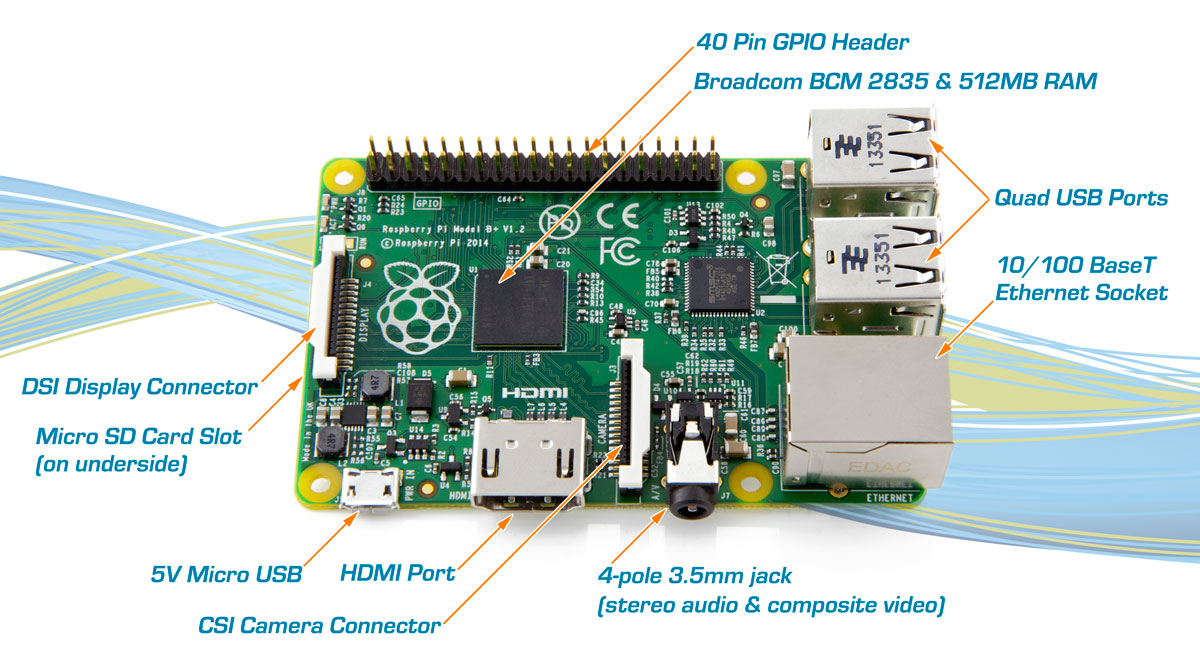
\includegraphics[scale=0.3]{Immagini/raspberry.png}
\caption{Raspberry PI 1 Model B+}
\end{figure}

\subsection{Perchè Raspberry}

Come già descritto nel capitolo \ref{chap:intro}, il prodotto che dobbiamo realizzare non solo deve essere in grado di far girare un webserver, ma deve anche essere in grado di comunicare con il mondo esterno. Raspberry Pi si è rilevato perfetto per questo scopo.
Essendo un dispositivo low cost che però ha sia un processore discreto che la possibilità di comunicare con relè e sensori, in quanto è dotato di ben 40 GPIO.